\chapter{Autonomous Search}
\label{chap:autonomous}

\section{Algorithm Selection and Autonomous Solvers}
\label{sec:algselres}

In 1976 John R. Rice published \textit{The Algorithm
Problem}~\cite{rice1976algorithm}, an influential paper where he formulated
abstract models for the problem of selecting effective algorithms for a given
problem. In Rice's framework the objective is to select the best algorithm,
according a performance metric, for a given problem. Consider a \textit{problem
space} $P$, and a problem $x \in P$.

Figure~\ref{fig:riceframe} presents Rice's algorithm selection
framework.

\begin{figure}[htpb]
    \begin{center}
        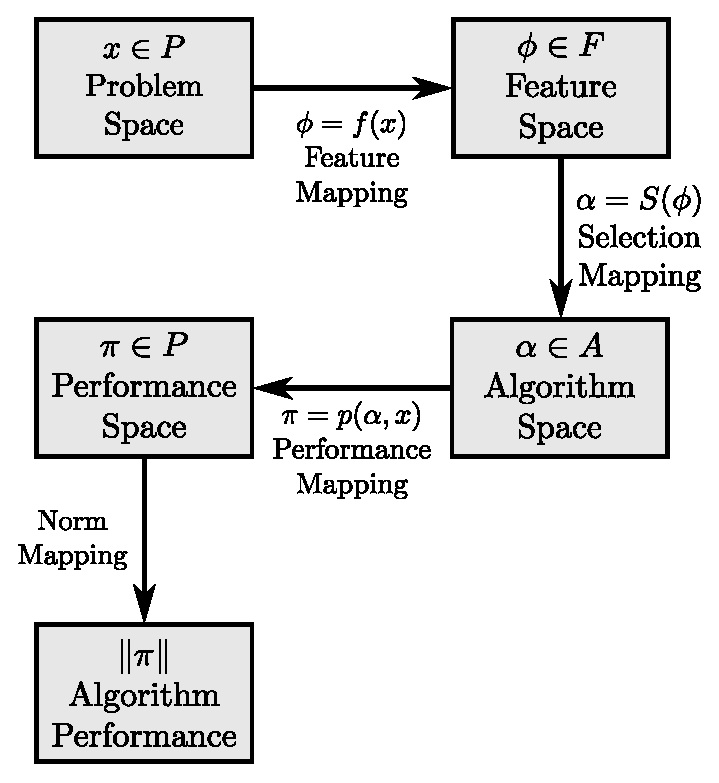
\includegraphics[width=.35\textwidth]{algorithm-selection}
    \end{center}
    \caption{Rice's framework}
    \label{fig:riceframe}
\end{figure}

\todo[inline,author=Pedro,color=cyan]{Discuss autonomous solvers}
\todo[inline,author=Pedro,color=cyan]{Discuss the choice of autotuning for
this work, given all the possibilities for solving the same problem
presented in this chapter}

\section{Off-line Configuration}
\label{sec:offconfig}

\subsection{Evolutionary Computing}
\label{subsec:evolcomp}

\subsection{Stochastic Local Search}
\label{subsec:searchsls}

\subsection{Machine Learning}
\label{subsec:searchml}

\section{On-line Control}
\label{sec:oncontrol}

\subsection{Adaptive Parameter Configuration}
\label{subsec:paramadaptive}

\subsection{Credit Assignment}
\label{subsec:creditassign}

\subsection{Reinforcement Learning}
\label{subsec:reinforce}
